\documentclass[12pt]{article}
\usepackage[utf8]{inputenc}
\usepackage[T1]{fontenc}
\usepackage{hyperref}
\usepackage{lipsum} % for placeholder text, remove if not needed
\usepackage[a4paper, portrait, margin=1.5cm]{geometry}
\usepackage{graphicx}
\usepackage{fancyhdr}
\usepackage{float}
\usepackage{color}
\definecolor{orange}{rgb}{1,0.5,0}


\title{IBM AI AR techdoc}
\author{Ani Bitri}

\begin{document}

\maketitle

\tableofcontents
\newpage

\section{Problem Statement}

    \subsection{Introduction and Context}

        Technical documentation plays a critical role in helping developers understand, implement, operate and maintain software systems. In enterprise environments, documentation is the primary interface between developers and complex
        systems, making clarity and accessibility essential. However, despite its importance, technical documentation remains predominantly static, text-based and difficult to navigate. As systems grow in complexity, dynamic processes such
        as data flows, dependencies and interactions are often poorly represented in traditional documentation formats. Consequently, many users often struggle to find the information they need, leading to frustration, errors and inefficiencies. This 
        raises the need for innovative solutions that can enhance the user experience and improve comprehension of technical documentation.

    \subsection{Existing Technologies}

    There are several existing technologies which address parts of the problem but do not yet offer a comprehensive solution. These include:
        \begin{itemize}
            \item \textbf{Static and Web-Based Documentation:}
                Different Platforms like GitBook, ReadTheDocs and Markdown-based tools offer well-structured and accessible documentation but lack interactivity and visualization capabilities. Information is conveyed effectively through text and images
                but remains static and fails to envision the dynamic nature of modern software systems.
            \item \textbf{AI Assistants:}
                In the last few years, the rise of AI-powered assistants like ChatGPT and Gemini have been transformative. These tools can understand and interpret technical text, summarize content and answer user queries. Yet, these
                assistants operate in isolation from the documentation itself, requiring users to switch contexts and manually input queries, disconnecting them from visual elements and offering limited support for the understanding of
                system architecture and interactions.
            \item \textbf{Augmented Reality Applications:}
                Industrial AR tools, such as PTC Vuforia, Microsoft Dynamics 365 Guides and Scope AR, have been used to overlay digital information onto real-world objects. These solutions enhance spatial understanding and are particularly useful in maintenance
                and training contexts. However, they typically rely on specific and expensive hardware, such as the HoloLens, or complex 3D models, thus limiting their accessibility for general users.
        \end{itemize}

    \subsection{Gaps in Current Solutions}

        Despite the advancements in AR and AI technologies, the current solutions exhibit several limitations:
        \begin{itemize}
            \item \textbf{Lack of Integration between AR and AI:}
                Visualization (AR) and comprehension (AI) are treated as separate domains. There is limited integration or implementation that combines the strengths of both to deliver a seamless user experience.
            \item \textbf{Limited Visual Comprehension:}
                Text and 2D diagrams are insufficient for conveying complex interactions and dynamic processes. Current documentation formats do not effectively utilize visual aids to enhance understanding.
            \item \textbf{Hardware and Platform Barriers:}
                Most AR implementations are dependent on specialized hardware, such as the HoloLens or AR glasses, which are costly or not widely available. This restricts the accessibility of AR-enhanced documentation to a broader audience.
        \end{itemize}

    \subsection{Problem Definition}

    Given the limitations of existing documentation systems and the potential of emerging technologies, there is a need for an innovative solution which can be easily accessible, interactive and capable of enhancing
    the understanding of technical documentation. In order to address this need, the project aims to develop an AI-powered mobile application that uses AR technology to augment technical documentation. The proposed system must 
    allow users to point their mobile devices at a technical diagram and view interactive AR overlays that explain components, relationships and interactions. At the same time, an integrated AI assistant, IBM Watson/Granite,
    will be available to answer user queries and provide additional context.  

        Therefore, this project aims to bridge the gap between visual comprehension and intelligent interaction in technical documentation, ultimately demonstrating how static documents can become interactive, explainable and user-friendly.


\section{Project Overview}

    \subsection{Purpose}
    Many developers face challenges while reading and understanding technical documentation. This project aims to create an AI-powered mobile application which, supported by AR technology, will enhance the user experience
    by providing interactive and immersive documentation. Powered by IBM Watson/Granite, the app will offer several features to assist developers in navigating and comprehending complex technical documents, including text recognition,
    interactive AR overlays, chatbot assistance and more.

    \subsection{Objectives within the scope}
    The primary objectives of this project are to:
    \begin{enumerate}
        \item Implement AR diagram augmentation
        \begin{itemize}
            \item Detect and track diagrams in printed and digital forms.
            \item Overlay interactive elements on diagrams to provide additional context and explanations.
        \end{itemize}
        \item Integrate an AI assistant
        \begin{itemize}
            	\item Employ IBM Watson/Granite to interpret the scanned documentation text and answer user queries.
            	\item Support natural language questions such as "What is the purpose of this diagram?" or "Explain this concept in simpler terms.".
        \end{itemize}
    \item Preserve accessibility and compliance
        \begin{itemize}
            \item Keep the core document unchanged and externalize enhancements through AR overlays to comply with accessibility and legal requirements.
        \end{itemize}
        \item Develop a functional mobile prototype
        \begin{itemize}
            \item Deliver a working mobile application prototype that demonstrates the key features and functionalities.
            \item Conduct user testing to gather feedback and refine the application.
            \item Provide a short demonstration.
        \end{itemize}
        \end{enumerate}

    \subsection{Boundaries and Out-of-Scope Elements}
    To keep the project achievable within the given timeframe, the following elements are considered out of scope:
    \begin{itemize}
        \item Full production deployment or enterprise-level integration.
        \item Hardware-specific AR is excluded; the focus is on mobile devices.
        \item Cross-platform optimization beyond the primary target platform (e.g., iOS or Android).
    \end{itemize}

    \subsection{Expected Deliverables}
    \begin{itemize}
        \item A prototype mobile application demonstrating real-time recognition and overlay of technical documentation.
        \item Integrated AI assistant interface capable of answering user queries based on the documentation content.
        \item A comprehensive project report detailing the design, implementation, testing processes and evaluation results.
        \item VIVA presentation and demonstration.
    \end{itemize}

    \subsection{Target Outcomes}
    \begin{itemize}
        \item Enhanced user experience for developers interacting with technical documentation.
        \item Improved comprehension of complex technical concepts through interactive AR elements and AI assistance.
        \item A foundation for future development and potential commercialization of the application.
    \end{itemize}

\section{Requirements}
Each requirement will be described in the format R{n}C/D, where n is the requirement number and C or D indicates whether the requirement is customer (C) or developer (D) oriented. For example,
R1C refers to the first customer requirement, while R2D refers to the second developer requirement. Each requirement will be detailed with its description, priority, verification method and traceability.

    \subsection{Functional Requirements}
    List the key functionalities the software system must support. Provide clear and concise descriptions of features and interactions.

    \begin{enumerate}
        \item \textbf{Augmented Reality System}
    \end{enumerate}

    \subsection{Non-Functional Requirements}
    Outline performance, usability, reliability, and other quality attributes expected from the system.

\section{System Architecture}
Provide a high-level overview of the system architecture. Include diagrams where appropriate to illustrate the system components and their interactions.

    \subsection{Design Pattern}

    The design pattern which will be adopted for this project is the Model-View-ViewModel (MVVM) pattern. This pattern is well-suited for applications that require a clear separation
    of concerns between the user interface and logic, making it easier to manage and test the application. Furthermore, the MVVM pattern facilitates a more modular and maintainable
    codebase, which is essential for the iterative development process planned for this project. The image below illustrates the MVVM architecture which will be used in the project.

    \begin{figure}[H]
        \centering
        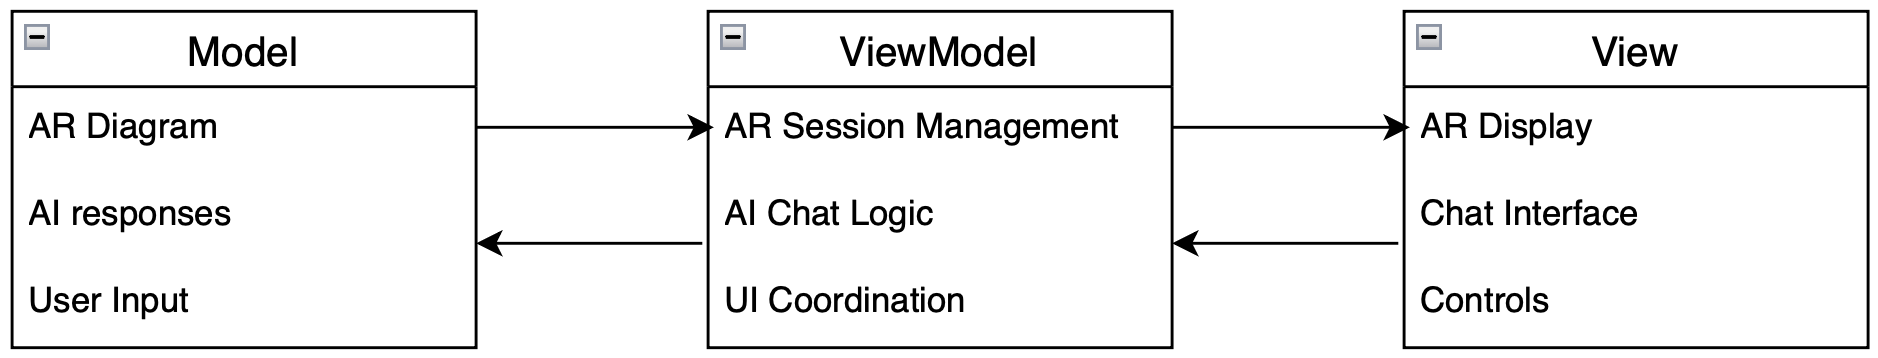
\includegraphics[width=\textwidth]{Pattern.png}
        \caption{MVVM Architecture Pattern}
        \label{fig:Pattern}
    \end{figure}

    \subsection{Frontend Design}

    \subsubsection{User Interface and User Experience}

        The application will feature a user-friendly interface that allows users to easily navigate through the app and access its features. The UI will be designed to be intuitive and responsive, ensuring a seamless user experience. When the user open the app, they will be presented with
        a simple home screen with options to scan a document, upload a document or access the history of previously scanned documents. Besides the home screen, the app will also include a tab for the chatbot, where users can interact with the AI assistant, and a settings tab for configuring
        app preferences. The image below illustrates the proposed UI design for the application:

        % UI image here

        Upon selecting the scan option, the user will be directed to the camera interface, where they can capture pictures of the technical documentation. Alternatively, the user can choose to upload the document from their device's storage and access the same features. After scanning or uploading
        a document, the app will process the text, images and diagrams, and give the user the option to view the AR overlays or interact with the AI assistant. The AR overlays will provide interactive elements that explain components, relationships and interactions within the diagrams based on the user's
        input and the information extracted from the document. The image below illustrates a flow chart of the app's user interface and navigation:

        % Flowchart image here
    \subsubsection{Error Handling and Feedback}

        To ensure a smooth user experience, the application will include robust error handling mechanisms. Internal errors will be handled gracefully and automatically, with appropriate messages displayed to the user upon interruptions. For example, if the app fails to recognize a diagram or if the AI assistant
        cannot process a query, the user will be informed of the issue and provided with suggestions for resolution. External errors will be handled by providing informative error messages to guide users in case of issues such as failed scans or uploads, network connectivity problems or AR tracking errors. Furthermore,
        error prevention strategies will be implemented to minimize their occurrence and impact on the user experience. Such strategies include input validation, network status checks and AR tracking optimizations. This approach will ensure that users can effectively utilize the app's features without being hindered by technical issues.



    \subsubsection{Integration with Backend and Data Flow}

        The frontend of the application will communicate with the backend services to process the scanned or uploaded documents and retrieve relevant information. The data flows as follows:
        \begin{enumerate}
            \item The user scans or uploads a document using the app's interface.
            \item The frontend validates the input and sends the document data to the backend for processing.
            \item The validated data is sent to the backend services for text recognition, diagram analysis and AI processing.
            \item The backend processes the data and generates AR overlays and AI responses based on the document content.
            \item The generated AR overlays and AI responses are sent back to the frontend for display to the user.
            \item The user interacts with the AR overlays and AI assistant, and any further queries or actions are sent back to the backend for processing.
        \end{enumerate}
        
    \subsection{Backend Design}

        \subsubsection{}

        \subsubsection{}

        \subsubsection{}

    \subsection{Technology Stack}
        The project will utilize the following technologies:
        \begin{itemize}
            \item \textbf{Frontend:} React Native for cross-platform mobile development, ARCore/ARKit/ViroReact for augmented reality functionalities.
            \item \textbf{Backend:} Node.js with Express for server-side logic, IBM Granite 4.0 for AI capabilities, IBM Granite Vision for image recognition, and MongoDB for data storage.
            \item \textbf{Development Tools:} Visual Studio Code for code editing, Git for version control, REST APIs for communication between frontend and backend.
        \end{itemize}

\section{Development Plan and Project Philosophy}

    \subsection{Methodology}

    Given the dynamic nature of the project and the need for iterative development, the Scrum framework within the Agile methodologies will be adopted. The approach will allow for flexibility, continuous feedback
    and incremental delivery of features. Weekly stand-up meetings will be held to discuss progress and address any challenges. The work will be organized into sprints, each lasting approximately one to two weeks,
    with clearly defined goals. At the end of each sprint, a review session will be held with the assessors to demonstrate progress and gather feedback.

    \subsection{Time Management and Milestones}
        The Gantt chart below outlines the planned work schedule, including key milestones and deadlines. Weekly meetings with the assessors will also be scheduled to ensure alignment and address any issues promptly.

        \begin{figure}[H]
        \centering
        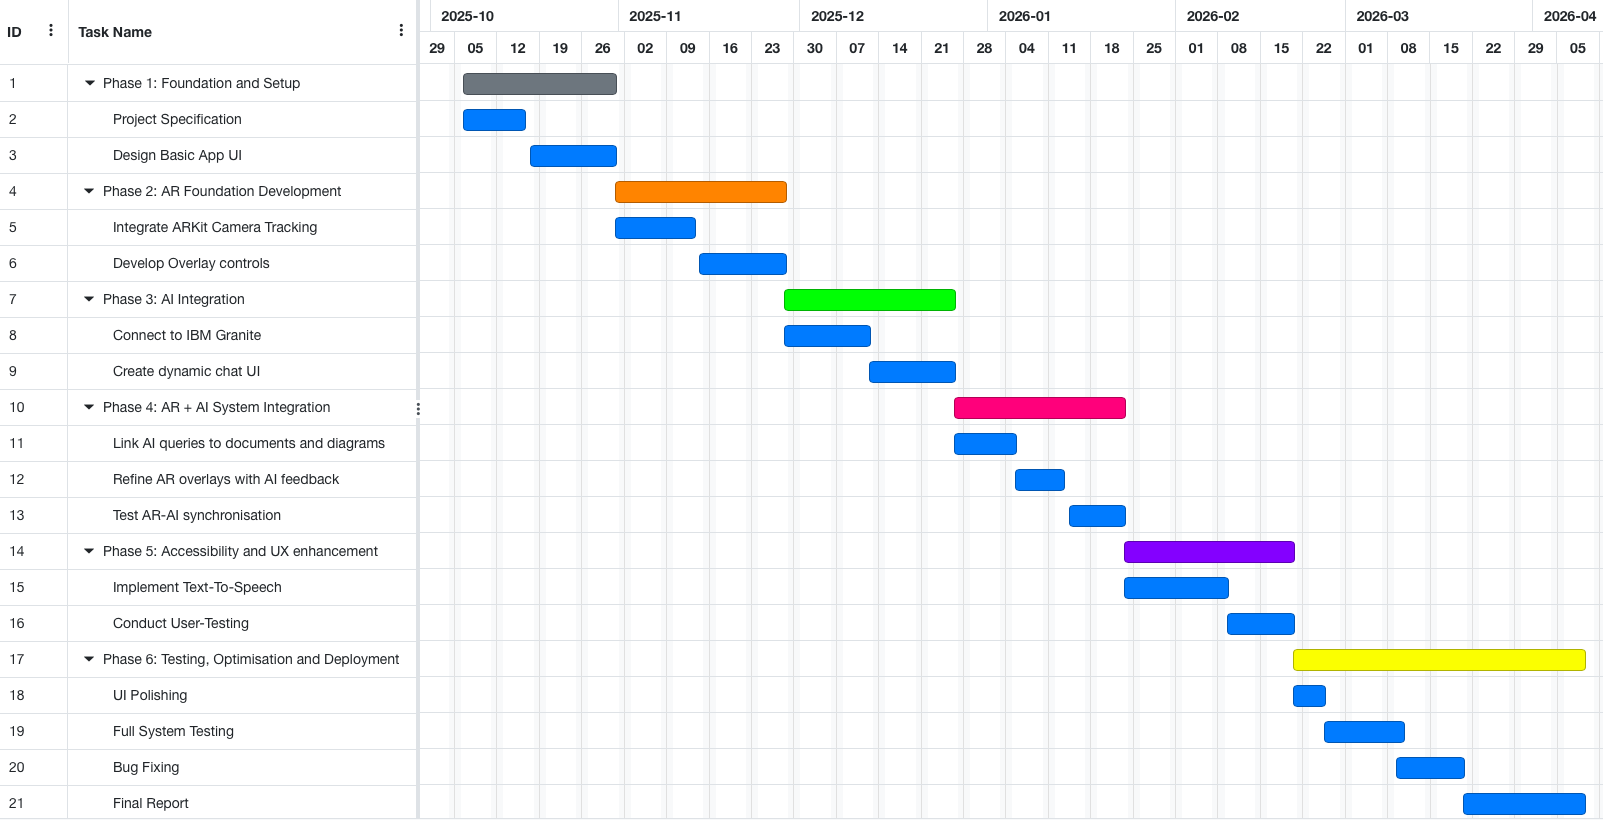
\includegraphics[width=\textwidth]{GanttChart.png}
        \caption{Gantt Chart of Planned Work Schedule}
        \label{fig:GanttChart}
        \end{figure}

    \subsection{Resource Management}

    The project will be primarily developed by a single developer, with support and guidance from the assessors. The developer will be responsible for all aspects of the project, including design, implementation, testing and documentation.
    Access to the essential software tools and platforms, such as IBM Granite and IBM Cloud, will be provided by IBM. Other resources, such as hardware for testing, necessary software and other materials, will be handled by the developer. Except for the
    resources provided by IBM, the developer will be responsible for acquiring any additional resources needed for the successful completion of the project. In the case of any type of resource unavailability, such as laptop malfunction or equipment failure, the
    developer will rely on the university's resources provided to students.


    \subsection{Risk Management}
    The following risks have been identified for the project, along with their descriptions, risk levels, likelihoods and mitigation strategies.
        \subsubsection{Technology Limitations}
        \begin{itemize}
            \item Risk description: There is unfamiliarity with some tools, libraries, or frameworks, which may cause delays or reduced performance. 
            \item Risk Level: \textcolor{green}{Tolerable}
            \item Risk Likelihood: \textcolor{orange}{Moderate}
            \item Mitigation Strategy: Conduct thorough research and allocate time for learning and experimentation with new technologies.
        \end{itemize}

        \subsubsection{Rollback Challenges}
        \begin{itemize}
            \item Risk description: Lack of a version control system could prevent from rolling back to the software's last stable state in case of errors
            \item Risk Level: \textcolor{red}{Catastrophic}
            \item Risk Likelihood: \textcolor{green}{Low}
            \item Mitigation Strategy: Utilise github to always maintain a stable version of the software and updating it when being sure that the changes will not affect its usability. 
        \end{itemize}

        \subsubsection{Testing Risks}
        \begin{itemize}
            \item Risk description: Insufficient testing may reduce confidence in the software
            \item Risk Level: \textcolor{orange}{Serious}
            \item Risk Likelihood: \textcolor{orange}{Moderate}
            \item Mitigation Strategy: Unit tests will be designed to test the software to make sure that it is working properly and user testing will be conducted to gather feedback and identify any issues.
        \end{itemize}

        \subsubsection{Time Management}
        \begin{itemize}
            \item Risk description: Underestimating  task duration or improper prioritization might result in delayed work.
            \item Risk Level: \textcolor{orange}{Serious}
            \item Risk Likelihood: \textcolor{green}{Low}
            \item Mitigation Strategy: Meetings with the assessors will be held weekly to ensure that the project is on track and any issues are addressed promptly.
        \end{itemize}

        \subsubsection{Requirement Misalignment}
        \begin{itemize}
            \item Risk description: During the development of the software, the end product might not be the same as the one described in the deliverables due to unforeseen circumstances.
            \item Risk Level: \textcolor{red}{Catastrophic}
            \item Risk Likelihood: \textcolor{green}{Low}
            \item Mitigation Strategy: Regular meetings with the assessors will be held to ensure that the project is on track and any issues are addressed promptly.
        \end{itemize}

        \subsubsection{Underestimating Sprint Workload}
        \begin{itemize}
            \item Risk description: Tasks may take longer than expected due to AI and AR complexities, which may lead to incomplete sprints and delays.
            \item Risk Level: \textcolor{orange}{Serious}
            \item Risk Likelihood: \textcolor{orange}{Moderate}
            \item Mitigation Strategy: Buffer time will be allocated in each sprint to accommodate unforeseen challenges, and tasks will be prioritized to ensure critical features are completed first.
        \end{itemize}

\section{Conclusion}
Summarize the key points of the specification document and outline next steps.

\end{document}